% 第十六章：贝塞尔函数\index{贝塞尔函数}

\chapter{贝塞尔函数\index{贝塞尔函数}}

\begin{wulibj}[本章导读]
贝塞尔函数\index{贝塞尔函数}是求解柱坐标系下数学物理方程时出现的特殊函数。它们在物理学中有广泛应用，如圆形膜的振动、圆柱形波导中的电磁场、量子力学中的二维谐振子等。本章我们将学习贝塞尔函数\index{贝塞尔函数}的定义、性质及其应用。
\end{wulibj}

% ========== 第一节 ==========
\section{贝塞尔方程的导出}

\subsection{柱坐标系下拉普拉斯方程的分离变量}

在柱坐标系 $(r, \varphi, z)$ 中，拉普拉斯方程为
\begin{equation}
    \frac{1}{r}\frac{\partial}{\partial r}\left(r\frac{\partial u}{\partial r}\right) + \frac{1}{r^2}\frac{\partial^2 u}{\partial\varphi^2} + \frac{\partial^2 u}{\partial z^2} = 0
\end{equation}

设 $u(r, \varphi, z) = R(r)\Phi(\varphi)Z(z)$，分离变量：

$\varphi$ 方向（周期性条件）：
\begin{equation}
    \Phi'' + m^2\Phi = 0 \quad \Rightarrow \quad \Phi = \mathrm{e}^{im\varphi}
\end{equation}

$z$ 方向：
\begin{equation}
    Z'' - k^2 Z = 0 \quad \Rightarrow \quad Z = \mathrm{e}^{\pm kz}
\end{equation}

$r$ 方向（设 $x = kr$）：
\begin{equation}
    \boxed{x^2\frac{\mathrm{d}^2 R}{\mathrm{d}x^2} + x\frac{\mathrm{d}R}{\mathrm{d}x} + (x^2 - m^2)R = 0}
\end{equation}

这就是 $m$ 阶\textbf{贝塞尔方程}。

% ========== 第二节 ==========
\section{贝塞尔函数\index{贝塞尔函数}的定义}

\subsection{第一类贝塞尔函数\index{贝塞尔函数} $J_m(x)$}

\begin{zhongyao}[第一类贝塞尔函数]
\[
    J_m(x) = \sum_{k=0}^{\infty} \frac{(-1)^k}{k!\Gamma(m+k+1)}\left(\frac{x}{2}\right)^{m+2k}
\]
\end{zhongyao}

前几项：
\begin{align}
    J_0(x) &= 1 - \frac{x^2}{4} + \frac{x^4}{64} - \frac{x^6}{2304} + \cdots \\
    J_1(x) &= \frac{x}{2} - \frac{x^3}{16} + \frac{x^5}{384} - \cdots
\end{align}

\begin{figure}[htbp]
\centering
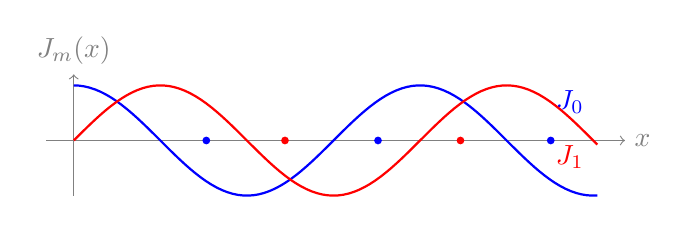
\begin{tikzpicture}[scale=0.7]
    \draw[->, gray] (-0.5, 0) -- (10, 0) node[right] {$x$};
    \draw[->, gray] (0, -1) -- (0, 1.2) node[above] {$J_m(x)$};
    
    % J_0
    \draw[blue, thick, domain=0:9.5, samples=100] plot (\x, {cos(deg(\x))});
    \node[blue] at (9, 0.7) {$J_0$};
    
    % J_1
    \draw[red, thick, domain=0:9.5, samples=100] plot (\x, {sin(deg(\x))});
    \node[red] at (9, -0.3) {$J_1$};
    
    % 零点标记
    \foreach \x in {2.405, 5.520, 8.654} {
        \fill[blue] (\x, 0) circle (2pt);
    }
    \foreach \x in {3.832, 7.016} {
        \fill[red] (\x, 0) circle (2pt);
    }
\end{tikzpicture}
\caption{贝塞尔函数\index{贝塞尔函数} $J_0(x)$ 和 $J_1(x)$}
\label{fig:bessel-functions}
\end{figure}

\subsection{第二类贝塞尔函数\index{贝塞尔函数} $Y_m(x)$}

\begin{dingliyi}{}{第二类贝塞尔函数}
贝塞尔方程的另一个线性无关解是\textbf{第二类贝塞尔函数\index{贝塞尔函数}}（诺伊曼函数）：
\begin{equation}
    Y_m(x) = \frac{J_m(x)\cos m\pi - J_{-m}(x)}{\sin m\pi}
\end{equation}

当 $m$ 为整数时取极限。
\end{dingliyi}

\begin{tishi}
$Y_m(x)$ 在 $x = 0$ 处发散，因此对于包含原点的区域，只使用 $J_m(x)$。
\end{tishi}

% ========== 第三节 ==========
\section{贝塞尔函数\index{贝塞尔函数}的性质}

\subsection{递推公式}

\begin{dingli}{}{递推公式}
\begin{align}
    \frac{\mathrm{d}}{\mathrm{d}x}[x^m J_m(x)] &= x^m J_{m-1}(x) \\
    \frac{\mathrm{d}}{\mathrm{d}x}[x^{-m} J_m(x)] &= -x^{-m} J_{m+1}(x) \\
    J_{m-1}(x) + J_{m+1}(x) &= \frac{2m}{x}J_m(x) \\
    J_{m-1}(x) - J_{m+1}(x) &= 2J_m'(x)
\end{align}
\end{dingli}

\begin{proof}
由贝塞尔函数的级数表示：
\begin{equation}
    J_m(x) = \sum_{k=0}^{\infty} \frac{(-1)^k}{k!\Gamma(m+k+1)}\left(\frac{x}{2}\right)^{m+2k}
\end{equation}

\textbf{第一式}：直接对 $x^m J_m(x)$ 求导：
\begin{equation}
    \frac{\mathrm{d}}{\mathrm{d}x}[x^m J_m(x)] = \sum_{k=0}^{\infty} \frac{(-1)^k(m+2k)}{k!\Gamma(m+k+1)}\left(\frac{x}{2}\right)^{m+2k-1}
\end{equation}
注意到 $(m+2k)/\Gamma(m+k+1) = 1/\Gamma(m+k)$，得 $x^m J_{m-1}(x)$。

\textbf{第二式}：类似地对 $x^{-m} J_m(x)$ 求导。

\textbf{第三、四式}：由第一、二式消去导数项得到。
\end{proof}
\subsection{渐近行为}

\begin{dingli}{}{渐近公式}
\begin{align}
    J_m(x) &\sim \frac{1}{\Gamma(m+1)}\left(\frac{x}{2}\right)^m, \quad x \to 0 \\
    J_m(x) &\sim \sqrt{\frac{2}{\pi x}}\cos\left(x - \frac{m\pi}{2} - \frac{\pi}{4}\right), \quad x \to \infty
\end{align}
\end{dingli}

\begin{proof}
\textbf{$x \to 0$ 的渐近式}：由级数展开，首项主导：
\begin{equation}
    J_m(x) = \frac{1}{\Gamma(m+1)}\left(\frac{x}{2}\right)^m \left[1 + O(x^2)\right]
\end{equation}

\textbf{$x \to \infty$ 的渐近式}：用最速下降法或鞍点法分析贝塞尔方程。设 $J_m(x) = y(x)/\sqrt{x}$，代入贝塞尔方程得：
\begin{equation}
    y'' + \left(1 - \frac{m^2 - 1/4}{x^2}\right)y = 0
\end{equation}
当 $x \to \infty$ 时，$y'' + y \approx 0$，故 $y \sim A\cos(x + \phi)$。确定相位后得渐近公式。

严格证明需用积分表示和鞍点法。
\end{proof}
\begin{wulibj}[物理意义]
大 $x$ 时的渐近行为表明 $J_m(x)$ 类似于衰减的余弦函数。这意味着贝塞尔函数\index{贝塞尔函数}描述的是衰减振荡。
\end{wulibj}

\subsection{零点}

贝塞尔函数\index{贝塞尔函数}有无限多个正零点，记为 $\mu_{m,n}$（$J_m(x)$ 的第 $n$ 个正零点）。

\begin{table}[htbp]
\centering
\begin{tabular}{cccc}
\toprule
$m$ & $\mu_{m,1}$ & $\mu_{m,2}$ & $\mu_{m,3}$ \\
\midrule
0 & 2.405 & 5.520 & 8.654 \\
1 & 3.832 & 7.016 & 10.174 \\
2 & 5.136 & 8.417 & 11.620 \\
\bottomrule
\end{tabular}
\caption{$J_m(x)$ 的前几个零点}
\end{table}

\subsection{正交性}

\begin{zhongyao}[贝塞尔函数的正交性]
设 $\mu_{m,n}$ 是 $J_m(x)$ 的第 $n$ 个零点，则
\[
    \int_0^1 xJ_m(\mu_{m,n}x)J_m(\mu_{m,n'}x)\,\mathrm{d}x = \frac{1}{2}[J_{m+1}(\mu_{m,n})]^2\delta_{nn'}
\]
\end{zhongyao}

更一般地，对于零点或边界条件导出的本征值：
\begin{equation}
    \int_0^a rJ_m\left(\frac{\mu_{m,n}r}{a}\right)J_m\left(\frac{\mu_{m,n'}r}{a}\right)\,\mathrm{d}r = \frac{a^2}{2}[J_{m+1}(\mu_{m,n})]^2\delta_{nn'}
\end{equation}

\subsection{傅里叶-贝塞尔级数}

任何满足适当条件的函数 $f(r)$ 可以展开为贝塞尔函数\index{贝塞尔函数}级数：
\begin{equation}
    f(r) = \sum_{n=1}^{\infty} c_n J_m\left(\frac{\mu_{m,n}r}{a}\right), \quad 0 \leq r \leq a
\end{equation}

其中
\begin{equation}
    \boxed{c_n = \frac{2}{a^2J_{m+1}^2(\mu_{m,n})}\int_0^a rf(r)J_m\left(\frac{\mu_{m,n}r}{a}\right)\,\mathrm{d}r}
\end{equation}

% ========== 第四节 ==========
\section{变形贝塞尔函数\index{贝塞尔函数}}

\subsection{变形贝塞尔方程}

将贝塞尔方程中的 $x$ 换成 $ix$，得
\begin{equation}
    x^2\frac{\mathrm{d}^2 y}{\mathrm{d}x^2} + x\frac{\mathrm{d}y}{\mathrm{d}x} - (x^2 + m^2)y = 0
\end{equation}

\subsection{第一类变形贝塞尔函数\index{贝塞尔函数}}

\begin{dingliyi}{}{第一类变形贝塞尔函数}
\begin{equation}
    \boxed{I_m(x) = \mathrm{i}^{-m}J_m(\mathrm{i}x) = \sum_{k=0}^{\infty} \frac{1}{k!\Gamma(m+k+1)}\left(\frac{x}{2}\right)^{m+2k}}
\end{equation}
\end{dingliyi}

$I_m(x)$ 在 $x \to \infty$ 时指数增长。

\subsection{第二类变形贝塞尔函数\index{贝塞尔函数}}

\begin{dingliyi}{}{第二类变形贝塞尔函数}
\begin{equation}
    K_m(x) = \frac{\pi}{2}\frac{I_{-m}(x) - I_m(x)}{\sin m\pi}
\end{equation}
\end{dingliyi}

$K_m(x)$ 在 $x \to \infty$ 时指数衰减，$x \to 0$ 时发散。

\begin{wulibj}[应用]
变形贝塞尔函数\index{贝塞尔函数}用于求解涉及径向变化的问题，如圆柱形导体中的稳恒电流分布、反应堆中的中子通量分布等。
\end{wulibj}

% ========== 第五节 ==========
\section{应用实例}

\subsection{圆形膜的振动}

\begin{lizi}{}{}
求半径为 $a$ 的圆形膜的振动，边界固定。

\begin{jie}
    振动方程：
    \begin{equation}
        u_{tt} = c^2\left(u_{rr} + \frac{1}{r}u_r + \frac{1}{r^2}u_{\varphi\varphi}\right)
    \end{equation}
    
    分离变量 $u(r, \varphi, t) = R(r)\Phi(\varphi)T(t)$。
    
    $R$ 满足贝塞尔方程，边界条件 $R(a) = 0$。
    
    本征值：$k_{m,n} = \mu_{m,n}/a$。
    
    固有频率：$\omega_{m,n} = c\mu_{m,n}/a$。
    
    本征函数：
    \begin{equation}
        u_{m,n}(r, \varphi, t) = J_m\left(\frac{\mu_{m,n}r}{a}\right)\begin{pmatrix}
            \cos m\varphi \\
            \sin m\varphi
        \end{pmatrix}\begin{pmatrix}
            \cos\omega_{m,n}t \\
            \sin\omega_{m,n}t
        \end{pmatrix}
    \end{equation}
\end{jie}
\end{lizi}

% ========== 本章小结 ==========
\section{本章小结}

\subsection{核心内容}

\begin{enumerate}
    \item 贝塞尔方程：$x^2y'' + xy' + (x^2 - m^2)y = 0$
    \item 第一类贝塞尔函数\index{贝塞尔函数}：$J_m(x) = \sum_{k=0}^{\infty} \frac{(-1)^k}{k!\Gamma(m+k+1)}(x/2)^{m+2k}$
    \item 正交性：$\int_0^1 xJ_m(\mu_{m,n}x)J_m(\mu_{m,n'}x)\,\mathrm{d}x \propto \delta_{nn'}$
    \item 变形贝塞尔函数\index{贝塞尔函数}：$I_m(x)$、$K_m(x)$
\end{enumerate}

\subsection{应用}

\begin{itemize}
    \item 圆柱坐标系下偏微分方程的分离变量
    \item 圆形膜的振动
    \item 圆柱形波导中的电磁场
    \item 热传导和扩散问题
\end{itemize}

% ========== 习题 ==========
\section{习题}

\textbf{基础题}

\begin{enumerate}
    \item 写出 $J_0(x)$ 和 $J_1(x)$ 的级数展开式的前四项。
    
    \item 利用递推公式证明 $J_0'(x) = -J_1(x)$。
    
    \item 计算 $J_2(x)$ 在 $x = 0$ 处的值。
\end{enumerate}

\textbf{综合题}

\begin{enumerate}[resume]
    \item 将函数 $f(r) = 1$（$0 \leq r \leq a$）展开为零阶贝塞尔函数\index{贝塞尔函数}级数（傅里叶-贝塞尔级数）。
    
    \item 求圆柱形区域 $r < a$ 内拉普拉斯方程的解，边界条件 $u(a, \varphi) = \sin 3\varphi$。
    
    \item 求圆形膜振动的前三个固有频率（已知 $J_0$ 的前三个零点）。
\end{enumerate}

\textbf{挑战题}

\begin{enumerate}[resume]
    \item 研究贝塞尔函数\index{贝塞尔函数}在光学衍射理论中的应用（圆孔衍射，Airy 斑）。
    
    \item 推导贝塞尔函数\index{贝塞尔函数}的积分表示：$J_m(x) = \frac{1}{2\pi}\int_{-\pi}^{\pi} \mathrm{e}^{\mathrm{i}(x\sin\theta - m\theta)}\,\mathrm{d}\theta$。
\end{enumerate}
